%\chapter*{Operational Requirements}\addcontentsline{toc}{chapter}{Operational Requirements}
\section{Operational Requirements}

V\& V has become a very popular concept recently, but has always been a vital process in the development of mission-critical systems. Losing or sinking the prototype due to faulty design or construction would have a devastating effect on my thesis, therefore I treated the system as mission-critical, trying to ensure very high reliability.

\subsection{General requirements of autonomus vehicles}

\subsection{Requirements of survey ships}

In order to execute a rational oceanography task, a number of valid objectives must be set. These objectives are usually one or more of the following\cite{oceanography}:

\begin{itemize}
\item A set of geographical measurement locations, with or without time and measurement type conditions
\item A certain area of interest
\item Maximal action duration requirement
\item Other
\end{itemize}

The task planning is usually carried out by the scientist group, but some auto-planning modes need to be supported. A typical task is the creation of a measurement-grid, with preset definition, in a certain geographical area. The High Level Controller (HLC) uses a Mission planning time algorithm, to support the auto-generation of the waypoints. This module is the "Waypoint planner", which outputs a list of coordinates that contains the measurement points.

Once the ship reaches the current waypoint, it determines the next aim.

A set of points defining a path can be specified for the ship, but it does not ensure that the created path is valid, therefore a second "Pathplanning" stage is required, which analyzes the generated set of locations and creates a path that is actually sailable by the ship.

\subsection{Combined requirements}

Validation requirements of the system:

\begin{itemize}

\item The robot can of navigate along a specified path
\item The robot can map a set of points in a given map
\item The robot can always find it’s way, if there exists any

\end{itemize}

Verification requirements of the control system:

\begin{itemize}

\item The controller can process sensor data into valid state readings
\item The controller ensures the asymptotic stability of the closed-loop system 

\end{itemize}

\begin{figure}[H]
	\centering
	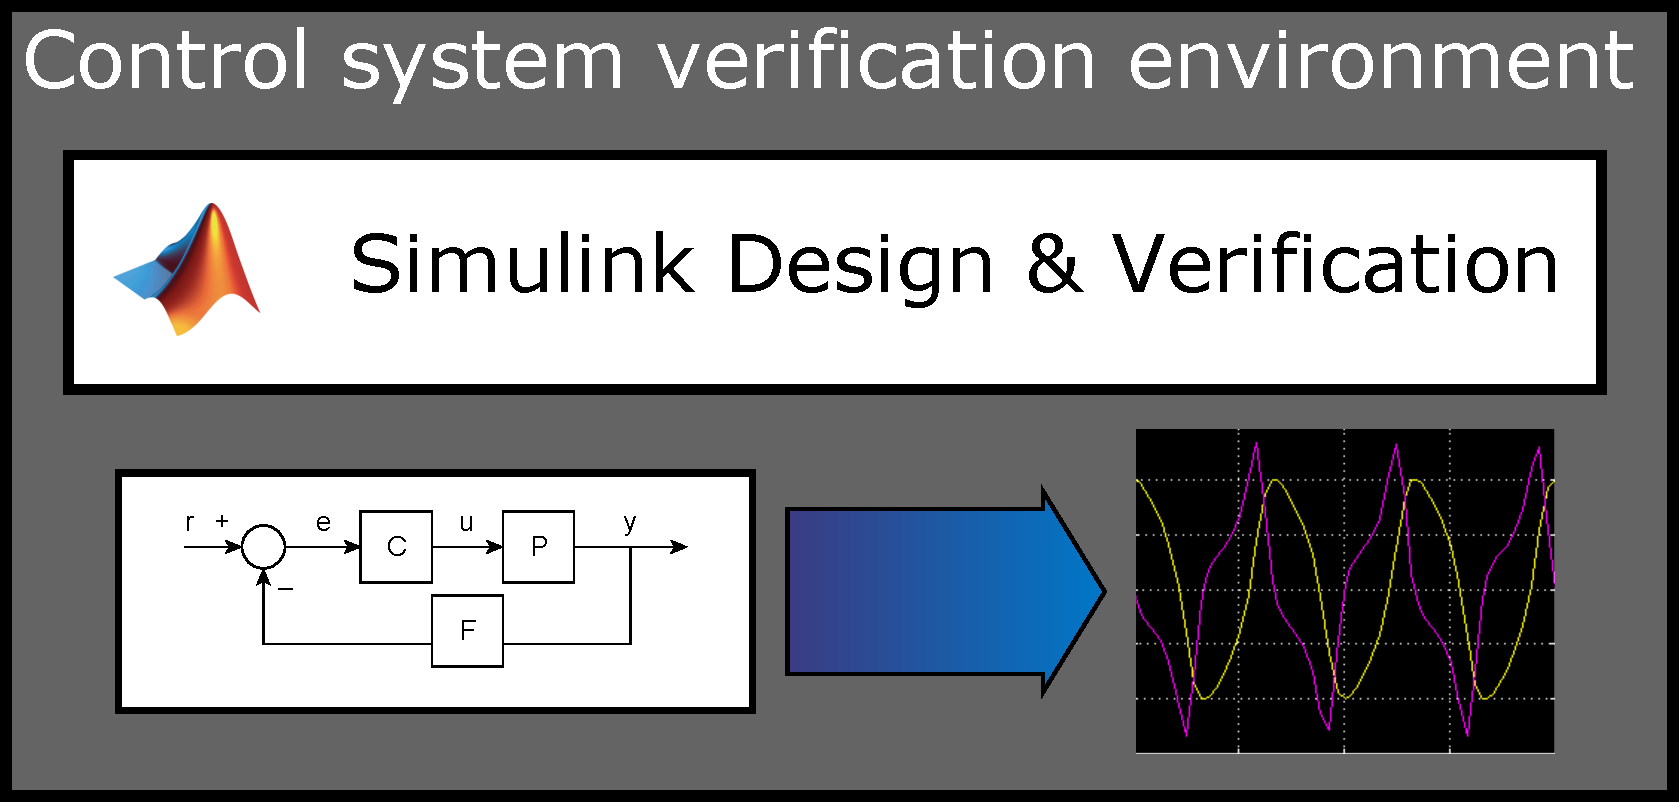
\includegraphics[width=0.8\textwidth]{img2/SimVer}
	\caption{}
	\label{}
\end{figure}

Verification requirements of the communication:

\begin{itemize}

\item The system can transmit and receive serial Bluetooth data
\item The system can process the incoming data
\item The system can automatically re-establish connection with the slave Bluetooth devices (GPS and client)
\item The system shuts down after a time period if connection was lost

\end{itemize}

\subsection{Verification requirements of the client software}

\begin{itemize}

\item The system can transmit and receive serial Bluetooth data
\item The system can provide valid real-time information about the system
\item The system can automatically re-establish connection with the master Bluetooth device (HLI)

\end{itemize}

\begin{figure}[H]
	\centering
	
\includegraphics[width=0.6\textwidth]{img2/VeriBadges}
	\caption{}
	\label{}
\end{figure}

\subsection{Validation of the system}

After the verification for the communication and the client software has finished, the validation process can begin. The validation consists of an outer simulation environment that tests the complete system. During the validation procedure a possible map and other mission parameters are supplied to the system, and the system response is evaluated.

\begin{figure}[H]
	\centering
	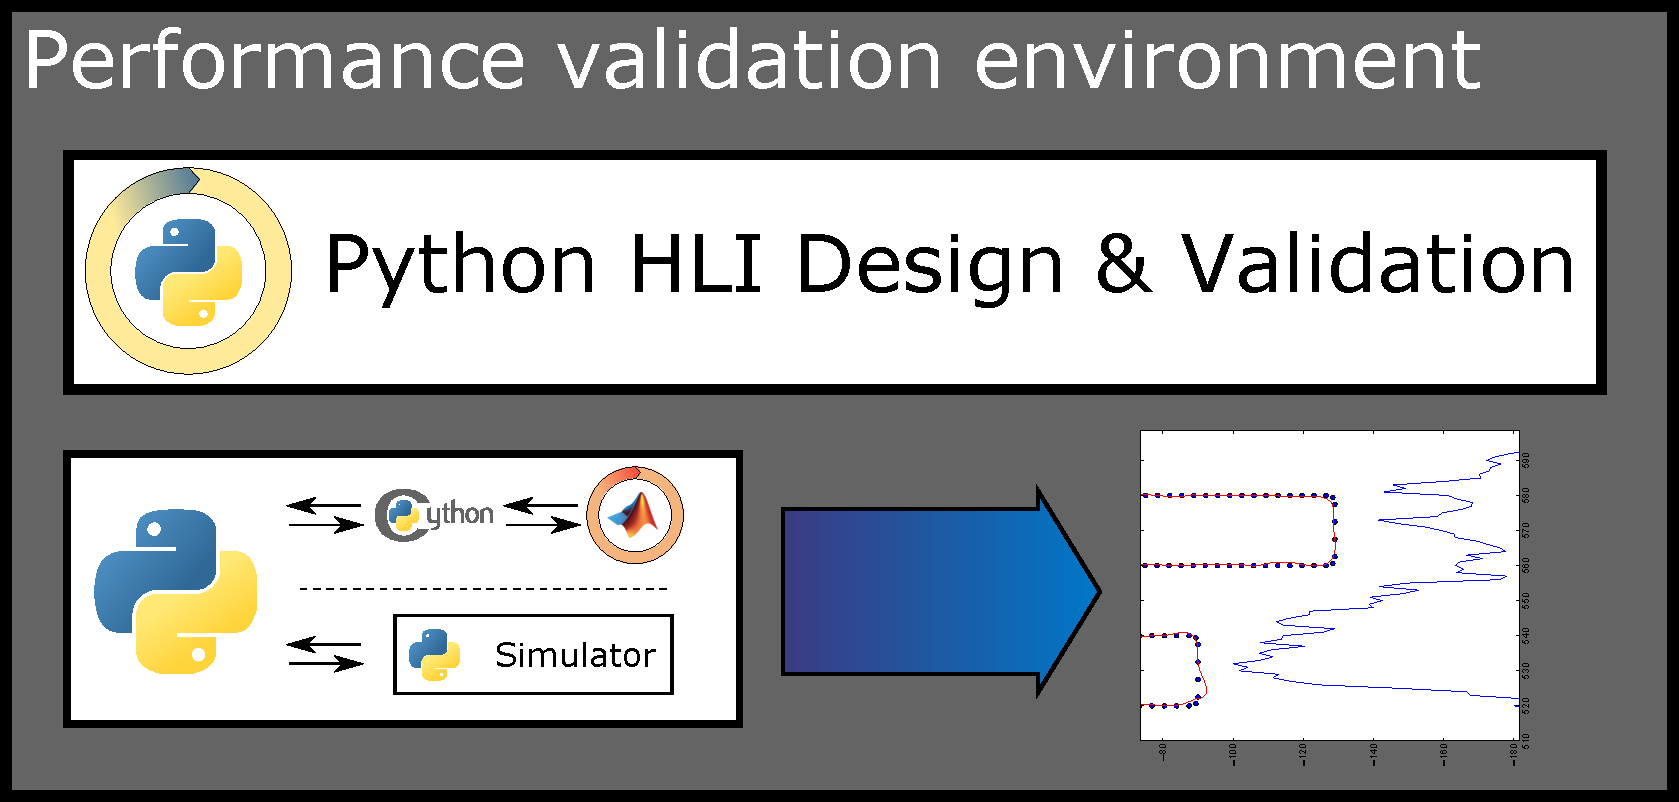
\includegraphics[width=0.8\textwidth]{img2/HLIVali}
	\caption{}
	\label{}
\end{figure}

\paragraph{Validation results} are not complete yet, only preliminary validation results are available from the previous semester. Along with the implementation of the client software, the validation procedure has the highest priority.